%% LaTeX2e class for student theses
%% sections/content.tex
%% 
%% Karlsruhe Institute of Technology
%% Institute for Program Structures and Data Organization
%% Chair for Software Design and Quality (SDQ)
%%
%% Dr.-Ing. Erik Burger
%% burger@kit.edu
%%
%% Version 1.1, 2014-11-21

%To be able to reference labels in other file
\externaldocument{introduction}
\externaldocument{appendix}


\chapter{Experimental Setup}
\label{ch:LITasks}

This chapter lays out the experimental setup used in this thesis. While Language Identification is applicable in many different scenarios, here the focus lies on trying to establish a low-latency online approach for recognizing the spoken language in a university-lecture environment. Because finding a suitable test setup for online data retrieval is hard, the data used was cut to short lengths to make an evaluation as to correctness of the recognition possible in an ''online-like'' scenario. 
This means that the output of the net is evaluated after short samples of speech and therefore can be seen as indicative of online performance of the net in the Lecture Translator. The test setup will be introduced in chapter~\ref{ch:eval}


This chapter introduces our experimental setup and tooling, and gives an overview of the used data sets.

\section{Language Identity Neural Networks}
\label{sec:LITasks:GS}

As this thesis continues the work of~\cite{Mueller2016b}, the experimental setup stayed mostly similar. After extraction of the audio features, as further described in Ch.~\ref{ch:FP}, we get a feature vector of 702, consisting of a combination of IMel and tonal features with a context of 6 frames as input and CD phoneme states as targets. This was trained in the mentioned previous work in a multilingual fashion, meaning it consists of multiple output layers, one for each layer.

The second last layer is the bottleneck layer (referring to a layer with a much smaller size than the previous and following one) with a size of 42. We then use the Bottleneck activations in training for the LID Neural Network. These BNF Vectors are stacked with a context to provide the input for the 2\textsuperscript{nd} LID network, as language identity is considered to be a long-term property of the audio data. We tried different context sizes (see sec.~\ref{sec:LIDNetwork:Input}), choosing the most robust one.  In opposition to the previous work mentioned where another BNF layer was introduced in the LID network to reuse the BNF vector in speech recognition tasks, we then use the output layer of the 2\textsuperscript{nd} layer to determine the language of the audio. This means the output layer consists of as many output neurons as available languages.

 fig.~\ref{fig:overview} gives an overview of this setup.

\tikzstyle{layer}=[draw=black,fill=black!30]
\tikzstyle{layerlid}=[draw=black,fill=green!30]
\tikzstyle{dots}=[draw=black,fill=black]
\begin{figure*}[htbp]
   \centering

   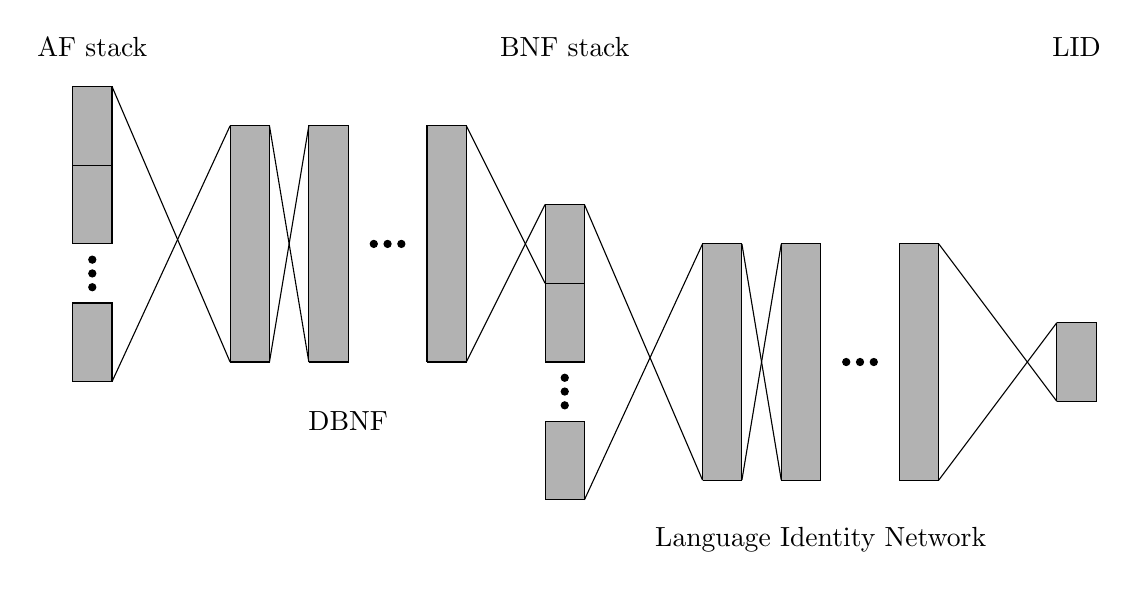
\begin{tikzpicture}[scale=1.0]

   % Acoustic feature stack

   \draw (-1.75, 2.5) node[draw=white,fill=white] {AF stack};

   \fill[layer] (-2,1) coordinate(l0bl) -- (-1.5,1) coordinate(l0br) --
(-1.5,2) coordinate(l0tr) -- (-2,2) coordinate(l0tl) -- (-2,1);

   \fill[layer] (-2,0) coordinate(l0_1bl) -- (-1.5,0) coordinate(l0_1br)
-- (-1.5,1) coordinate(l0_1tr) -- (-2,1) coordinate(l0_1tl) -- (-2,0);

   \draw[dots] (-1.75,-0.2) circle (0.045);
   \draw[dots] (-1.75,-0.375) circle (0.045);
   \draw[dots] (-1.75,-0.55) circle (0.045);

   \fill[layer] (-2,-1.75) coordinate(l0_2bl) -- (-1.5,-1.75)
coordinate(l0_2br) -- (-1.5,-0.75) coordinate(l0_2tr) -- (-2,-0.75)
coordinate(l0_2tl) -- (-2,-1.75);

   % Bottle-neck stack

   \fill[layer] (4,-1.5) coordinate(l5_1bl) -- (4.5,-1.5)
coordinate(l5_1br) -- (4.5,-0.5) coordinate(l5_1tr) -- (4,-0.5)
coordinate(l5_1tl) -- (4,-1.5);

   \draw[dots] (4.25,-1.7) circle (0.045);
   \draw[dots] (4.25,-1.875) circle (0.045);
   \draw[dots] (4.25,-2.05) circle (0.045);

   \fill[layer] (4,-3.25) coordinate(l5_2bl) -- (4.5,-3.25)
coordinate(l5_2br) -- (4.5,-2.25) coordinate(l5_2tr) -- (4,-2.25)
coordinate(l5_2tl) -- (4,-3.25);

   \draw (1.5,-2.25) node {DBNF};

   \draw (4.25,2.5) node[draw=white,fill=white] {BNF stack};

   % BNF Layers

   \fill[layer] (4,-0.5) coordinate(l5bl) -- (4.5,-0.5) coordinate(l5br)
-- (4.5,0.5) coordinate(l5tr) -- (4,0.5) coordinate(l5tl) -- (4,-0.5);
   \fill[layer] (2.5,-1.5) coordinate(l4bl) -- (3,-1.5) coordinate(l4br)
-- (3,1.5) coordinate(l4tr) -- (2.5,1.5) coordinate(l4tl) -- (2.5,-1.5);

   \draw[dots] (2,0) circle (0.045);
   \draw[dots] (2.175,0) circle (0.045);
   \draw[dots] (1.825,0) circle (0.045);

   \fill[layer] (1,-1.5) coordinate(l2bl) -- (1.5,-1.5) coordinate(l2br)
-- (1.5,1.5) coordinate(l2tr) -- (1,1.5) coordinate(l2tl) -- (1,-1.5);
   \fill[layer] (0,-1.5) coordinate(l1bl) -- (0.5,-1.5) coordinate(l1br)
-- (0.5,1.5) coordinate(l1tr) -- (0,1.5) coordinate(l1tl) -- (0,-1.5);

   \draw (l0tr) -- (l1bl);
   \draw (l0_2br) -- (l1tl);
   \draw (l1tr) -- (l2bl);
   \draw (l1br) -- (l2tl);
   \draw (l4tr) -- (l5bl);
   \draw (l4br) -- (l5tl);


   % DNN Layers

   \fill[layer] (6,-3) coordinate(l6bl) -- (6.5,-3) coordinate(l6br) --
(6.5,0) coordinate(l6tr) -- (6,0) coordinate(l6tl) -- (6,-3);
   \fill[layer] (7,-3) coordinate(l7bl) -- (7.5,-3) coordinate(l7br) --
(7.5,0) coordinate(l7tr) -- (7,0) coordinate(l7tl) -- (7,-3);

   \draw[dots] (8,-1.5) circle (0.045);
   \draw[dots] (8.175,-1.5) circle (0.045);
   \draw[dots] (7.825,-1.5) circle (0.045);

   \fill[layer] (8.5,-3) coordinate(l11bl) -- (9,-3) coordinate(l11br)
-- (9,0) coordinate(l11tr) -- (8.5,0) coordinate(l11tl) -- (8.5,-3);
   \fill[layer] (10.5,-2) coordinate(l12bl) -- (11,-2) coordinate(l12br)
-- (11,-1) coordinate(l12tr) -- (10.5,-1) coordinate(l12tl) -- (10.5,-1);

   \draw (10.75,2.5) node[draw=white,fill=white] {LID};

   \draw (l5tr) -- (l6bl);
   \draw (l5_2br) -- (l6tl);

   \draw (l6tr) -- (l7bl);
   \draw (l6br) -- (l7tl);
   \draw (l11tr) -- (l12bl);
   \draw (l11br) -- (l12tl);

   \draw (l12tl) -- (l12bl);

   \draw (7.5,-3.75) node {Language Identity Network};

   \end{tikzpicture}
   \caption{Overview of the network architecture used to extract
the Language Identity (LID). The acoustic features (AF) are being
pre-processed in a DBNF in order to extract BNFs. These BNFs are being
stacked and fed into the second network to extract the LID.}
   \label{fig:overview}
\end{figure*}

\section{Tooling}
\label{sec:tooling}

Many different tools exist for deep learning, the most acclaimed being Tensorflow~\cite{DBLP:journals/corr/AbadiABBCCCDDDG16}, DL4J/ND4j\footnote{DL4J:~\url{https://deeplearning4j.org/index.html}} and Theano~\cite{bergstra2011theano}. Pre-existing work on Language Identification, or rather Language Feature Vector Extraction using a LID Network in~\cite{Mueller2016b}, used a python wrapper around Theano for training, that was developed by Jonas Gehring~\cite{gehringMA}. This thesis continues the use of this wrapper for the training of our DNNs. The basic layout of the network used and improved upon by this thesis were input vectors from a multilingual ASR net, further explained in sec.~\ref{sec:FP:FA}, which we used to generate Bottleneck Features with 966 coefficients. The LID network introduced in the following chapters then uses these BNF vectors to classify the audio input into a language. Different Network Structures and types (DNNs/RNNs) were used that will be further explained in Ch.~\ref{ch:LIDNetwork}. 

As \texttt{detl} does not provide support for RNNs we used Lasagne~\footnote{Lasagne: \url{https://lasagne.readthedocs.io/en/latest/}}, another wrapper around Theano, as the framework for our RNN training.

\section{Euronews 2014}
\label{sec:LITasks:Euronews}


The first data set used, was retrieved from Euronews \footnote{Euronews: http://www.Euronews.com/} 2014. Euronews is a TV channel that is broadcast in 13 different languages simultaneously both on TV and over the Web and is semi-automatically transcribed. The data corpus includes 10 languages (Arabian, German, Spanish, French, Italian, Polish, Portuguese, Russian, Turkish and English) with around 72 hours of data per language provided overall, meaning the corpus had a total length of around 720 hours of audio data. This data was taken both from online video and recordings of the transmissions as described in \cite{gretter2014Euronews}.

For the purposes of this work we then broke this corpus down further into a more manageable size as to make the feedback-cycle faster, while still keeping the corpus big enough to make results comparable to performance with the full corpus. Later, we then used the full data set to compare results between the smaller and bigger sets.

The corpus was broken down to a per-speaker-basis based on its automatic transcriptions. From this data we took a sample of a random 10.000 speakers, while making sure the total length of samples for each language were roughly the same. Details of this breakdown can be seen in table ~\ref{tab:spkData}.

\begin{table}[h!]
\caption{The Euronews corpus speaker breakdown used for most experiments with total utterances length.}
\label{tab:spkData}
\centering
\begin{tabular}{| l | c | r | }
	\hline
	\textbf{Language} & \textbf{Number of Speakers} & \textbf{Combined Length} \\
	\hline
	Arabian & 1055 & 16.76 h \\
	German & 928 & 18.80 h \\
	Spanish & 932 & 18.78 h \\
	French & 1016 & 18.67 h \\  
	Italian & 935 & 19.00 h \\  
	Polish & 1229 & 18.30 h \\ 
	Portuguese & 1062 & 16.19 h \\ 
	Russian & 958 & 18.66 h \\ 
	Turkish & 957 & 18.61 h \\  
	English & 928 & 18.54 h \\ 
	\hline
	\textbf{Overall} & 10000 & 182.31 h\\
	\hline	
\end{tabular}
\end{table}

\begin{table}[h!]
\caption{The Euronews corpus breakdown into the three data sets.}
\label{tab:spkSplit}
\centering
\begin{tabular}{| l | c | r | }
	\hline
	\textbf{Set} & \textbf{Number of Speakers} & \textbf{Combined Length} \\
	\hline
	Train &  8000 & 149.76 h \\
	Development & 1000 & 19.46 h \\
	Test & 1000 & 19.29 h \\
	\hline
\end{tabular}
\end{table}

The speaker list was then split into three smaller datasets: the train set, development set and test set using the common Simple Random Sampling. The sizes were \(80\%\) allocated to the train set, and \(10\%\) to each the development and test set. Table~\ref{tab:spkSplit} shows the split data for the three sets. The development set will be referred to as DEV and the test set as TEST after this.

The complete Euronews Corpus available was much larger. This was used to confirm intuition that a larger data corpus leads to better results which can be seen in sec.~\ref{sec:LIDNetworkBig}. The breakdown of the large corpus' data is listed in table~\ref{tab:spkDataBig}.

\begin{table}[h!]
\caption{The full Euronews corpus speaker breakdown with total utterances length.}
\label{tab:spkDataBig}
\centering
\begin{tabular}{| l | c | r | }
	\hline
	\textbf{Language} & \textbf{Number of Speakers} & \textbf{Combined Length} \\
	\hline
	Arabian & 4401 & 51.13 h \\
	German & 4436 & 73.21 h \\
	Spanish & 4464 & 75.71 h \\
	French & 4434 & 68.14 h \\  
	Italian & 4464 & 77.22 h \\  
	Polish & 2625 & 33.15 h \\ 
	Portuguese & 4430 & 49.07 h \\ 
	Russian & 4418 & 72.23 h \\ 
	Turkish & 4385 & 70.42 h \\  
	English & 4511 & 72.76 h \\ 
	\hline
	\textbf{Overall} & 42568 & 643.04 h\\
	\hline	
\end{tabular}
\end{table}

\newpage
\section{Lecture Data}
\label{sec:LITasks:Lecture}

As part of the development of the KIT's Lecture Translator, German lectures at the KIT were recorded and annotated. This is described in~\cite{stuker2012kit}. This thesis then uses parts of this German corpus as well as newer recordings done at the KIT of English lectures with the same setup, English academic talks given at InterACT25\footnote{InterACT25: \url{http://www.interact25.org/}}, as well as French talks done at the DGA's~\footnote{DGA: \url{http://www.defense.gouv.fr/dga}} yearly academic conference on speech recognition.

This lecture data was then used in two different ways: Firstly, to evaluate the 10-Language trained Euronews-Net(s) to see how it would fare in a lecture-environment as part of the KIT's Lecture Translator by scaling the output down to the 3 available languages. Secondly to train a second net and further test the findings about the net setup and net evaluation, as found with the Euronews corpus.

The breakdown of speakers and length can be seen in table~\ref{tab:spkDataLD}. As the main work was done on the Euronews corpus this data corpus is considerably smaller and was mostly just used as a proof-of-concept for a possible integration of a LID-Net into the Lecture Translator. 

The development set for the LD corpus consisted of 1.5h of Lecture Data per each of the three languages with one speaker for German/English (one class' recording) and 5 French speakers from DGA talks.
\begin{table}[h!]
\caption{The Lecture Data corpus speaker breakdown with total utterances length.}
\label{tab:spkDataLD}
\centering
\begin{tabular}{| l | c | r | }
	\hline
	\textbf{Language} & \textbf{Number of Speakers} & \textbf{Combined Length} \\
	\hline
	German & 8 &  16.22 h \\
	French & 30 & 8.25 h \\  
	English & 27 & 10.78 h \\ 
	\hline
	\textbf{Overall} & 65 & 35.25 h\\
	\hline	
\end{tabular}
\end{table}

\section{European Parliament}
\label{sec:LITasks:EU}

As another form of evaluation, recordings of the European Parliament speeches, that are freely available online~\footnote{EU-Parliament plenary speeches: \url{http://www.europarl.europa.eu/ep-live/en/plenary/}} were used. The video recordings come with the simultaneous translations into all the official languages of the EU-countries.  This includes seven of the languages also available on Euronews, namely German, English, French, Spanish, Italian, Polish and Portuguese. We extracted the seven audio tracks embedded in the recordings with ffmpeg~\footnote{ffmpeg:\url{https://ffmpeg.org/}}. The audio extracted is of the simultaneous translations with an underlying audio track of the original speaker, which adds noise, but is similar in nature to the Euronews recordings that often feature an underlying audio track in a different language.

The small corpus was used to evaluate performance of the Euronews-trained nets, as well as improve capabilities of the networks with cross-training on top of the Euronews-nets, of which results can be seen in the following chapter.

As each parliament discussion includes the same audio tracks, the length of all the languages in the set is the same, with each language having 3.6 hours of data. 

\chapter{Feature Preprocessing}
\label{ch:FP}

This chapter deals with the feature preprocessing used to form normal speech into feature vectors to be understood by neural networks. The setup used is based on the standard capabilities of the Janus Recognition Toolkit. The following sections describe this Feature Preprocessing for data as well as the first multilingual ASR network as introduced previously, used to create the BNF features the LID net requires.  It is based on preprocessing introduced in~\cite{Mueller2016b}.
Features produced by this preprocessing setup are then written to ``pfiles'' together with their labels (the target language). The pfiles are then used to train the network using detl, or, in the case of RNNs, lasagne by supervised training employing the Stochastic Gradient Descent with Newbob scheduling.

\section{Feature Retrieval}
\label{sec:FP:FA}
The audio files available to us in the Euronews and Lecture Data corpus were recorded using a sampling rate of 16 kHz. European Parliament data we collected ourselves were recorded with a sample rate of 44.1 kHz. We down-sampled the data using soX\footnote{soX Sound eXchange: \url{http://sox.sourceforge.net/}}. 
\paragraph{Full Euronews Corpus} The Full Euronews Corpus, as introduced in section~\ref{sec:LITasks:Euronews}, had prexisting pfiles from previous work~\cite{Mueller2016b} that we reused. This meant that the features in this case were completely based on 32ms windows and not a combination of 16ms and 32ms windows as for the rest of the corpora.

\section{Feature Description}
\label{sec:FP:FD}
For the DBNF network as input, a combination of sound power, lMEL, fundamental frequency variation (FFV)~\cite{laskowski2008fundamental}, \cite{laskowski2008fundamental} and pitch acoustic features~\cite{schubert1999grundfrequenzverfolgung} was used. Tonal features have shown improvements for DNNs, even with non-tonal languages as English~\cite{metze2013models}, so they were also incorporated. Lst.~\ref{lst:features} in the appendix shows the complete feature extraction source code in tcl.

Using the sound power feature that is part of Janus' standard capabilities, we added a speech-detection feature, which identifies speech and noise from the audio. We first calculate the \(log\) on the current sound power and then determine the weighted average with a context of 2 frames on each side. After normalizing the resulting value between -0.1 and 0.5, we apply a basic threshold function: We consider everything above 0 in the normalized spectrum as speech, and below as (non-speech) noise. We do not discard the non-speech marked parts however, but weigh the combined feature vector less in the resulting input vector for the neural network.

The log mel features are calculated the following way: We calculate the spectrum of the audio waveform using the Fast Fourier Transformation on 16 ms windows, calculate the Mel Coefficients, apply Vocal Tract Length Normalization (VTLN) on the spectrum in the linear domain and then multiply the Mel-Filterbank coefficients with the normalized coefficients. We apply a logarithm to this to get the lMEL features.

From Janus' standard pitch capability, calculated on 16 ms windows, we calculate the symmetric delta coefficients \((f(t+\delta) - f(t-\delta)\) on the pitch for \(\delta=1,2,3\) and the same deltas on those results and merge to give us a coefficients for frame t. This means we define:
\begin{equation}
f(t):=PITCH(t+1)-PITCH(t-1)
\end{equation}
\begin{equation}
g(t):=PITCH(t+2)-PITCH(t-2)
\end{equation}
\begin{equation}
h(t):=PITCH(t+3)-PITCH(t-3)
\end{equation}

Merging these we get the coefficients:
\begin{equation}
(PITCH(t),f(t),f(t+1)-f(t-1),g(t),g(t+2)-g(t-2),h(t),h(t+3)-h(t-3))
\end{equation}
The FFV is calculated on 32 ms windows, to then be merged  with the pitch feature we just defined to make up the TONE feature. lMEL coefficients and TONE coefficients are then merged. See~\cite{laskowski2009modeling},  \cite{laskowski2008fundamental}These feature vectors are stacked with a context of 6 adjacent frames and then passed to the DBNF net as introduced in the next section.
\paragraph{Full Euronews Corpus} The full Euronews corpus used 32 ms for all feature calculations, so the sound power, FFT/lMEL and pitch were calculated on 32ms windows, but used the same features aside from this.
\paragraph{Lecture Data/European Parliament} For the other two data corpora we kept the 16ms windows for power and lMEL, but changed the pitch to be calculated on 32 ms windows.

\section{DBNF network}
\label{sec:FP:Net}

The DBNF was trained as part of~\cite{Mueller2016b}. It is trained using the input features defined in section~\ref{sec:FP:FD}. The targets are context-dependent phoneme states, representing a similar setup to how an ASR neural network. The network has 6 layers of 1000 neurons each plus a bottleneck layer of 42 neurons before the final output layer. 

The activations of the bottleneck layer are extracted. We then apply a context of 11 frames and stack the frame itself with the context. The context is calculated using a spread of 3. This means we only use every 3\textsuperscript{rd} frame. The stacked vector is then used as the input for the LID network on which the following chapter will elaborate. 


\section{Evaluating Input Features}
\label{sec:LIDNetwork:Input}

Work in~\cite{Mueller2016b} included a comparison of different context spreads as stacked inputs for the LID net of 2,3 and 6. As one of the first experiments on the Euronews corpus we increased the spreads from 3 to 4 and 5 frames, while still keeping the original context width of 11 (meaning a total context width of 44 Frames (880ms) and 55 Frames (1100ms) respectively). This however proved not successful as performance decreased already in the frame-based metrics and was therefore likely to also decrease in the per-sample metric as introduced in the following chapter. 

For all further experiments on Network layout and smoothing, we therefore used the best performing context of 33, with a spread of 3 frames.

table~\ref{tab:resCtx} at the end of the next chapter shows the results for the different selected spreads with different net structures, which are introduced in the following chapter.

\chapter{LID Network Structure}
\label{ch:LIDNetwork}

This chapter describes the actual Language Identification neural networks trained as well as the results of different network/data setups used. Most network experiments in the network geometry, referring to the number of hidden layers as well as the layout of the neurons in these layers, were evaluated using the Euronews corpus. Results from this corpus were then transferred over to the other corpora, meaning that the network layout that worked best for Euronews was then adjusted for the lecture data but otherwise the geometry was kept intact.

\section{Baseline Setup}
\label{sec:LIDNetwork:Basic}

The first experimental net setup consisted of 5 layers of denoising auto-encoders. Each layer had 1000 nodes, aside from the input layer using the 966 feature frames that is the input vector whose contents were described in the previous chapter, and a \texttt{tanh} activation function using the mean squared error as the loss function. 

The neural net was then trained using mini batches of size 2,000,000. The training was done using a learning rate of 0.01. The pre-trained net was then retrained with a 1000 neuron to 10 coefficient output to get to our 10 Languages as classes to classify against. In the basic setup this was trained using a learning rate of 1 and the exit condition of a minimum change of 0.005 / 0.0001 for the training/validation data respectively.

The beginning benchmark to improve upon was then set to the frame-based validation/train error of 0.23 / 0.27 respectively, while of course understanding that non-training per-sample data would most likely have worse results at first than the frame-based validation error calculated on training data.

The following section describes different network layouts and changes we made to the training of the neural network and the improvements made upon our initial result.

\section{Improving Network Layout}
\label{sec:LIDNetwork:Layout}

Different network layout were tried and experimented with. This includes a 6 pre-trained hidden layer version, as well as changes in the geometry. The differences in the frame-based errors can be seen in table~\ref{tab:resFrameBased}. 

\paragraph{Decreasing Learning Rate} Setting the learning rate of the output layer training to 0.1 instead of the default 1, gave us the first increase in frame-based recognition rates, improving it from an error of 0.274 for the base setup to an error rate of only 0.256, giving an improvement of almost 2\%. As table~\ref{tab:resFrameBased} shows, the higher learning rate lead to a better train-set result but worse validation performance, this could be an indication that the lower learning rate stops the net from over-learning as much and increases generality.

\paragraph{Adding the 6th hidden layer} Adding another 1000 neuron hidden layer did not lead to an increase in recognition compared to the version using a lower learning rate and rather gave us an decrease of about 2\%, meaning an error rate of 0.275 compared to the 0.256 for the lower learning rate version.

\paragraph{``Tree'' net structure} The biggest increase was achieved by changing the geometry of the net from 5 layers with each 1000 neurons to one of each layer having 200 less neurons of the previous one giving us a net definition of (\texttt{tanh} being the activation function, \texttt{mse} the loss function of the mean squared error and make da the command for \texttt{detl} to add another hidden layer):

\begin{verbatim}'!make da 966,tanh:1000 loss=mse' \
  '!make da 1000:800' \
  '!make da 800:600' \
  '!make da 600:400' \
  '!make da 400:200' \
\end{verbatim}

This setup, with the standard output layer with 10 output neurons, improved error rates from 0.256 down to 0.245, an improvement of 1.2 \%.

Adding another 6th hidden layer onto this structure to give a net definition of (visualized in fig.~\ref{fig:treeNet}):
\begin{verbatim}'!make da 966,tanh:1200 loss=mse' \
  '!make da 1200:1000' \
  '!make da 1000:800' \
  '!make da 800:600' \
  '!make da 600:400' \
  '!make da 400:200' \
\end{verbatim}

further improved the results, yielding an error rate of only 0.241, performing another 0.4 \% better than the 5-layer tree-structure. 


\tikzstyle{layer}=[draw=black,fill=black!30]
\tikzstyle{layerlid}=[draw=black,fill=green!30]
\tikzstyle{dots}=[draw=black,fill=black]
\begin{figure*}[htbp]
   \centering
   \caption{Visualization of the tree-net structure.}
   \label{fig:treeNet}
   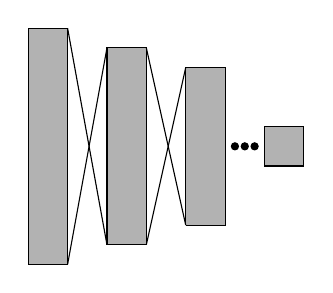
\begin{tikzpicture}[scale=1.0]


   \fill[layer] (0,-1.5) coordinate(l1bl) -- (0.5,-1.5) coordinate(l1br)
-- (0.5,1.5) coordinate(l1tr) -- (0,1.5) coordinate(l1tl) -- (0,-1.5);
   \fill[layer] (1,-1.25) coordinate(l2bl) -- (1.5,-1.25) coordinate(l2br)
-- (1.5,1.25) coordinate(l2tr) -- (1,1.25) coordinate(l2tl) -- (1,-1.25);
   \fill[layer] (2,-1.0) coordinate(l3bl) -- (2.5,-1.0) coordinate(l3br)
-- (2.5,1.0) coordinate(l3tr) -- (2,1.0) coordinate(l3tl) -- (2,-1.0);

   \draw[dots] (2.625,0) circle (0.045);
   \draw[dots] (2.75,0) circle (0.045);
   \draw[dots] (2.875,0) circle (0.045);


   \draw (l1tr) -- (l2bl);
   \draw (l1br) -- (l2tl);
   \draw(l2tr) -- (l3bl);
   \draw(l2br) -- (l3tl);

   \fill[layer] (3,-0.25) coordinate(l4bl) -- (3.5,-0.25) coordinate(l4br)
-- (3.5,0.25) coordinate(l4tr) -- (3,0.25) coordinate(l4tl) -- (3,-0.25);

 
   \end{tikzpicture}
\end{figure*}

A possible explanation for the better performance of the tree structure could be, that the farther the layer is removed from the input, it works on recognizing more ``abstract'' patterns, and less of the more abstract classes exist than of basic patterns. E.g. the first layer decides on the values of one certain frequency of the input what language is more likely, with the second layer then taking into account a whole range of frequencies (of which less exist) or even more abstract features to further differentiate.

Adding a larger number of hidden layers into this tree structure did not improve results, as a 10-hidden-layer version with the setup of:

\begin{verbatim}
 '!make da 966,tanh:2000 loss=mse' \
  '!make da 2000:1800' \
  '!make da 1800:1600' \
  '!make da 1600:1400' \
  '!make da 1400:1200' \
  '!make da 1200:1000' \
  '!make da 1000:800' \
  '!make da 800:600' \
  '!make da 600:400' \
  '!make da 400:200' \
\end{verbatim}

failed to perform featuring an error rate of 90 \%, meaning the net was not able to classify correctly anymore.

As deeper hidden layers will take longer/more data to train correctly (as the changes have to propagate through the earlier layers first, to then affect the deeper layers), our setup did most likely not include enough data for the training of these nets. Another explanation could be the spreading of information in the input 966 features onto the 2000 neurons of the first hidden layer added wrong coefficients.

Overall the tree-net with 5 layers and reduced learning rate performed the best in the frame-based errors, featuring a relative improvement of 0.175 compared to the basic net.

\begin{table}[h!]
\caption{Results of the different context sizes on the Euronews corpus for the first 3 introduced net structures. Frame-based errors on train/validation set.}
\label{tab:resCtx}
\centering
\begin{tabular}{| l | c | r | }
	\hline
	\textbf{Net Structure (context)} & \textbf{Train Error} & \textbf{Validation Error}  \\
	\hline
	Basic (33) & 0.226 &  0.285 \\
	\hline
	Basic (44) & 0.073 & 0.353 \\
	\hline
	Basic (55) & 0.209 & 0.309 \\
	\hline
	6-Layers (33) & 0.236 & 0.276 \\
	\hline
	6-Layers (44) & \textbf{0.192} & 0.326 \\
	\hline
	6-Layers (55) & 0.243 & 0.298 \\
	\hline
	Reduced Learning Rate (33) & 0.273 & \textbf{0.266} \\ 
	\hline
	Reduced Learning Rate (44) & 0.287 & 0.310 \\ 
	\hline
	Reduced Learning Rate (55) & 0.276 & 0.268 \\ 
	\hline
	\textbf{Best} & \textbf{0.192} & \textbf{0.266} \\
	\hline
\end{tabular}
\end{table}


\begin{table}[h!]
\centering
\caption{Results of the different net structures on the Euronews corpus. Frame-based errors on train/validation set.}
\label{tab:resFrameBased}
\begin{tabular}{| l | c | c | r |}
	\hline
	\textbf{Net Structure} & \textbf{Train Error} & \textbf{Val. Error}   & \parbox[t]{2cm}{\textbf{Rel. Impr.} \\ \textbf{Val. Error}} \\
	\hline
	Basic (5 layers 1000 Neurons) & 0.226 &  0.285 & -\\
	\hline
	6-Layers (1000 Neurons) & 0.236 & 0.276 & 0.032 \\
	\hline
	Reduced Learning Rate & 0.273 & 0.266 & 0.067 \\ 
	\hline
	\parbox[t]{5cm}{Tree Structure \\ (5 layers 1000...200 neurons)} & 0.221 & 0.245 & 0.140 \\
	\hline
	\parbox[t]{5cm}{Tree Structure \\ (5 layers 1000...200 neurons)\\and reduced learning rate} & 0.245 & \textbf{0.235} & \textbf{0.175} \\
	\hline
	\parbox[t]{5cm}{Tree Structure \\ (6 layers 1200...200 neurons)} & \textbf{0.211} & 0.242 & 0.151 \\
	\hline
	\parbox[t]{5cm}{Tree Structure (6 layers 1200...200 neurons) \\
	and reduced learning rate} & 0.251 & 0.238 & 0.164 \\
	\hline
	\parbox[t]{5cm}{Tree Structure \\ (7 layers 1400...200 neurons)} & 0.206 & 0.247 & 0.133 \\
	\hline
	\parbox[t]{5cm}{Tree Structure \\ (10 layers 2000...200 neurons)} & 0.899 & 0.910 & - \\
	\hline
	\textbf{Best} & \textbf{0.211} & \textbf{0.235} & \textbf{0.175} \\
	\hline
\end{tabular}
\end{table}

\section{Full Euronews Corpus}
\label{sec:LIDNetworkBig}

As introduced in sec.~\ref{sec:LITasks:Euronews}, a bigger Euronews data was used to further evaluate our network structure. The net was trained with the tree-net 6-layer structure with a reduced learning rate as introduced above. This resulted in a train error of 0.204 and a validation error of only 0.169, an improvement of 6.9\% compared to the smaller corpus with the same net structure. However, it only improved the error in classifying each sample of the DEV set (as further introduced in the next chapter) by about 4\%. As the amount of train data was trippled while the classification only improved by about 4 \%, this suggests that a suitable post-net filtering approach and net setup will have a bigger impact than the data corpus size after a certain threshold.

\begin{table}[h!]
\centering
\caption{Comparison of the big and small Euronews data corpus. Frame-based errors on train/validation set, as well as Sample-based Error.}
\label{tab:resBigNet}
\begin{tabular}{| l | c | c | r | }
	\hline
	\textbf{Data Corpus} & \textbf{Train Error} & \textbf{Validation Error} & \textbf{Sample Error} \\
	\hline
	Small (17h/Language) & 0.251 &  0.238 & 0.318 \\
	\hline
	Full (70h/Language) & 0.204 & 0.169 &  0.276 \\
	\hline
	\textbf{Change} & \color{green}{\textbf{0.047}} & \color{green}{\textbf{0.069}} & \color{green}{\textbf{0.042}} \\
	\hline
\end{tabular}
\end{table}

\section{Cross-set training}
\label{sec:LIDNetwork:Fine}
As a further experiment, we used the pre-trained nets of the stacked hidden layers of the Euronews net and trained the output layer on top with the cross-set of Lecture-Data. This was done by loading net-parameters from pre-training and training the final output layer with the cross-set on top of them. For the final layer we used a low learning rate of 0.1 (1/10th of the learning rate we used in the normal setup), to make meaningful learning possible while cross-training only the final layer.

As a basis for the cross-training, we loaded the tree-net 6-layer structure of the Euronews nets, omitting the output layer. We then used the lecture data corpus to train the output layer with only 3 output neurons. This yielded an improvement of 4.9\% for the error of the tree-net Euronews net recognizing the lecture data development set on a per-sample basis (for which the test setup is introduced in the next chapter).

A second experiment was conducted, using the same base Euronews net, but adding 2 layers on top for the cross-training with 200 and 100 neurons respectively, instead of only one output layer with 200:10 neurons. This further improved the Frame-based results, by another 1.4\%., and sample-based results by another 1.8\%. This gives us a total improvement of 6.7\% for the cross-training compared to the base Euronews net. See tab.~\ref{tab:LIDFine} for the detailed results.


Since the Lecture Data corpus only has 3 languages, we could not evaluate the cross-trained nets using all Euronews languages but still gave a figure for the net results with the Euronews corpus for English, German and French. These results are obviously much worse than pure-Euronews-trained nets, as the two output layers have never seen euronews data, that while similiar, is obviously still sufficiently different, as the performance suffered by 12.1\%.


\begin{table}
\caption{Results of the cross-training attempts of the Euronews-trained 6-layer tree-net with the lecture data (LD) corpus. 3 Languages (3L) are German, English, French.}
\label{tab:LIDFine}
\begin{tabular}{| l | c | c | c | r | }
	\hline
	\textbf{Net Structure} & \parbox[t]{2cm}{\textbf{Euronews} \\ \textbf{(DEV)} \\ \textbf{3L Error}} &  \parbox[t]{2.3cm}{\textbf{LD} \\ \textbf{Train} \textbf{Error}} &  \parbox[t]{2cm}{\textbf{LD} \\ \textbf{Val. Error}} &  \parbox[t]{2.5cm}{\textbf{LD} \\ \textbf{Sample Error}}  \\
	\hline
	\parbox[t]{4.2cm}{Tree-net Euronews net \\
	 w/o cross-training}  & 0.291 & - & - & 0.179 \\
	\hline
	\parbox[t]{4.2cm}{Tree-net Euronews net \\ with cross-training } & 0.456 & 0.075 & 0.116 & 0.130 \\
	\hdashline
	\parbox[t]{4.2cm}{Tree-net Euronews net \\ with cross-training 2 layers } & \textbf{0.413} & 0.073 & 0.102 & \textbf{0.112} \\
	\hline
	\textbf{Change (best)} & \color{red}{\textbf{0.121}} & - & - & \color{green}{\textbf{0.067}} \\
	\hline
\end{tabular}
\end{table}


\section{Combining Lecture Data and Euronews}
\label{sec:LIDNetworkConcat}
By combining both the lecture data and Euronews corpusses, we produced improved results that can be seen in Tab~\ref{tab:resultsLD}. This was to be expected just from the amount of train data almost doubling for the 3 lecture data-languages. Overall, this net produced the best results for the lecture data corpus by a big margin of 23 \%. The concateneted corpus also produced the best results on the Euronews corpus with an increase in the error of only 0.005 compared to the non-augmented Euronews data. 

\section{Lecture-Data-Training}
\label{sec:LIDNetworkLDTraining}

After trying cross-training and concatenation for the lecture data corpus, we also trained a net on the Lecture Data corpus. We continued the use of the tree-net structure as it had proven successful with the Euronews corpus. We first evaluated the same 6-layer setup with and without an adjusted learning rate. Additionally we also experimented with a smaller, 4-layer tree-net with a structure of:
\begin{verbatim}
  '!make da 966,tanh:800 loss=mse' \
  '!make da 800:600' \
  '!make da 600:400' \
  '!make da 400:200' \
\end{verbatim}

The 6-layer net did prove to perform better than the 4-layer one in the frame-based metric, and surprisingly in this case, the non-adjusted learning rate version (so the standard learning rate of 1.0) performed better than the lowered one, as the validation error of the 6-layer-standard-lr-net was about 0.6\% better than the version with the lowered learning rate for the LD Evaluation.  Overall however, the LD-Trained Net with 4 layers performed the best on full samples, the metric that can be most related to performance in an online fashion. This confirms our findings on the Euronews corpus of a tree-net structure performing the best for LID.

Suprisingly, the other ld-only nets did feature a better validation/train error frame-based but failed to achieve higher accuracy in sample-evaluation in comparison with the cross-trained versions. Possibly, this can be attributed to the fact that the lecture data corpus overall is much smaller than the Euronews one, on which the cross-trained version were pre-trained on, and therefore have less transferabilty.

table~\ref{tab:resultsLD} shows a comparison of the different Lecture Data experiments and a summary of the improvements we made. Overall the best net for lecture data would be the concatenated data corpus trained net with a sample error of only 0.65\%. However, zhe LD-only trained net with 4 layers and a tree-structure, is only 2.3\% worse than this net, while having a much smaller corpus size. 

Intuition dictates, that the cross-trained versions would perform better on the Euronews corpus than the ld-only trained ones, which was confirmed by the results. However, the difference in error was smaller than expected, with only 2.6\% between the best-performing LD-net and the cross-trained 2-layer net for the Euronews error.



\begin{table}
\caption{Results of the different lecture data (LD) approaches. 3 Languages (3L) are German, English, French.}
\label{tab:resultsLD}
\begin{tabular}{| l | c | c | c | r | }
	\hline
	\textbf{Net Structure} & \parbox[t]{2cm}{\textbf{Euronews} \\ \textbf{(DEV)} \\ \textbf{3L Error}} & \parbox[t]{2cm}{\textbf{LD} \\ \textbf{Train} \textbf{Error}} & \parbox[t]{2cm}{\textbf{LD} \\ \textbf{Val. Error}} & \parbox[t]{2.5cm}{\textbf{LD} \\ \textbf{Sample Error}} \\
	\hline
	\parbox[t]{4.2cm}{Tree-net Euronews net \\
	 w/o cross-training}  & 0.291 & - & - & 0.179 \\
	\hline
	\parbox[t]{4.2cm}{Concatenated \\ Euronews/LD-trained net } & \textbf{0.296} & 0.206 & 0.245 & \textbf{0.065} \\
	\hdashline
	\parbox[t]{4.2cm}{Tree-net Euronews net \\ with cross-training } & 0.456 & 0.075 & 0.116 & 0.130 \\
	\hdashline
	\parbox[t]{4.2cm}{Tree-net Euronews net \\ with cross-training 2 layers } & 0.413 & 0.073 & 0.102 & 0.112 \\
	\hdashline
	\parbox[t]{4.2cm}{LD-Trained Net 4 layers} & 0.438 & 0.076 & 0.109 & 0.088 \\
	\hdashline
	\parbox[t]{4.2cm}{LD-Trained-Net 6 layers} & 0.439 & 0.026 & 0.093 & 0.150 \\
	\hdashline
	\parbox[t]{4.2cm}{LD-Trained Net 6 layers \\ \& lowered learning rate} & 0.417 & 0.066 & 0.100 & 0.112 \\
	\hline
	\parbox[t]{4.2cm}{\textbf{Change} \textbf{(best)}} & \color{red}{\textbf{0.005}} & - & - & \color{green}{\textbf{0.114}} \\
	\hline
\end{tabular}
\end{table}

\section{European Parliament}
\label{sec:EP}

As to further test the conclusions made about net-structure/cross-training we also trained data on the small European Parliament corpus we collected. The setup was very similar to the Lecture Data tests as introduced in the previous section.  We however did not try to concatenate the train data with the other corpora available.

The two cross-training attempts had the same setup. For the EP-only training we found that the 6-layer tree-net structure performs worse than the base setup (5 layers with 1000 neurons each). This however could be due to the minimal data available in the EP corpus and the fact that less layers in this case would always perform better.

Surprisingly, even though the train data available was very small, the improvements in comparison to the Euronews net results for European Parliament speeches are still better by 2.6\%, showing that neural networks already start performing even with minimal data available and selection of train data similar to later actual input is very important. See table ~\ref{tab:resultsEP} for the summarized results. Overall it's clear, that the European parliament data is substantially different from the Euronews set up as the Euronews trained net performs worse even with cross-training than a net trained directly on the small Europearn Parliament corpus itself.


\begin{table}
\label{tab:resultsEP}
\caption{Results of the different European parliament (EP) approaches. 7 languages (7L) are German, French, Italian, English, Polish, Portuguese, Spanish}
\begin{tabular}{| l | c | c | c | r | }
	\hline
	\textbf{Net Structure} & \parbox[t]{2cm}{\textbf{Euronews (DEV)} \\  \textbf{7L Error}} & \parbox[t]{1.5cm}{\textbf{EP} \\ \textbf{Train Error}} & \parbox[t]{2cm}{\textbf{EP} \\ \textbf{Val. Error}} & \parbox[t]{2.5cm}{\textbf{EP} \\ \textbf{Sample Error}}  \\
	\hline
	\parbox[t]{4.2cm}{Tree-net Euronews net \\
	 w/o cross-training} & 0.297 & - & - & 0.383 \\
	\hline
	\parbox[t]{4.2cm}{Tree-net Euronews net \\ with cross-training } & \textbf{0.676} & 0.230 & 0.292 & 0.456 \\
	\hdashline
	\parbox[t]{4.2cm}{Tree-net Euronews net \\ with cross-training 2 layers } &  \textbf{0.676} & 0.267 & 0.310 & 0.391 \\
	\hdashline
	\parbox[t]{4.2cm}{EP-Trained Net 5 layers } & 0.679 & 0.155 & 0.333 & \textbf{0.357} \\
	\hdashline
	EP-Trained Net 6 layers & 0.691 & 0.061 & 0.361 & 0.392 \\
	\hline
	\parbox[t]{5cm}{\textbf{Change} \textbf{(best)}} & \color{red}{\textbf{0.379}} & - & - & \color{green}{\textbf{0.026}} \\
	\hline
\end{tabular}
\end{table}

\chapter{Smoothing and Evaluation}
\label{ch:eval}

While frame-based error rates on the training/validation sets were already sufficiently good from the LID networks, this of course is not a reliable indicator of real-world online performance, so the development setup consisted of (for each data corpus) a development set (as introduced in Ch.~\ref{ch:LITasks}) of speakers whose samples were run through the LID setup (Feature Preprocessing ch.~\ref{ch:FP}, DBNF extraction ch.~\ref{sec:FP:Net}. LID network ch.~\ref{ch:LIDNetwork}). The following smoothing approaches were applied in an ''online'' fashion, meaning it was made sure they can be calculated in real time while new data is still coming in. The summarized results are listed in tab.~\ref{tab:evalTotal},~\ref{tab:evalTotal2} for both the DEV and TEST results. We chose to only run the experiments on the Euronews corpus, as the 10-language-target will always have more possible erroneous outputs and filtering can prove to more successfull. We evaluated different net structures, however the results presented here are based on the tree-net 6-layer structure as introduced in the previous chapter. This is not necessarily the best structure for the frame-based train error, but it gave us the best results on a sample basis (see tab.~\ref{tab:evalNS}).

\section{Output Activations}
\label{sec:outputs}

We started by evaluating a few samples manually by looking at the output. In the following diagrams one row is equal to activation of one output neuron (bottom to top ID 0-9). Activations are marked black for high activations and white for low activations. The x-scale is the current frame number (with one frame being 10 ms long). As expected activations for random noise/music as in fig.~\ref{fig:noise} are smooth over all the frames and do not show any language as being predominant. 

Also, for a 800 ms Polish sample, fig.~\ref{fig:polish} shows the output activations for a correctly recognized sample. It is clear, that the language with ID 5 is the one being spoken in the sample as the 5th row in the picture has the highest activations. This is equal to Polish (as arbitrarily defined in the pfiles writing script). 

An incorrectly classified sample can be seen in fig.~\ref{fig:incorrect}. The language of the sample is English (ID 9), but from frame 50 on it is being (mostly) classified as Arabian (ID 0). However, one can also see, that the activations of the network are not smooth and tend to jump around as different languages appear as the maximum in this sample, e.g. also German (ID 1) appears to have high activations at different times. 

\begin{figure}[h!]
\caption{Activation of output neurons for random non-speech (jingles/noise)}
\label{fig:noise}
\centering
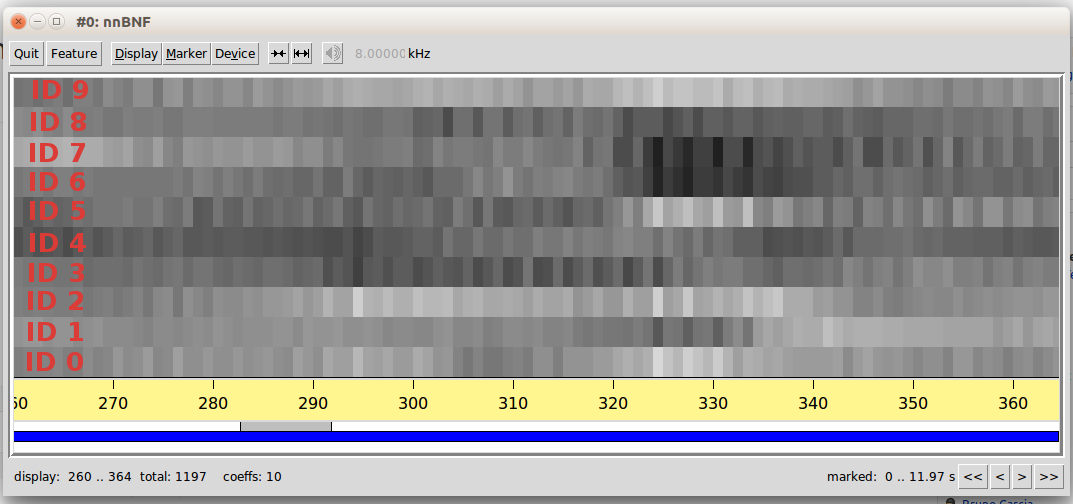
\includegraphics[width=0.7\textwidth]{images/noise.png}
\end{figure}

\begin{figure}[h!]
\caption{Activation of output neurons for a correctly recognized Polish sample}
\label{fig:polish}
\centering
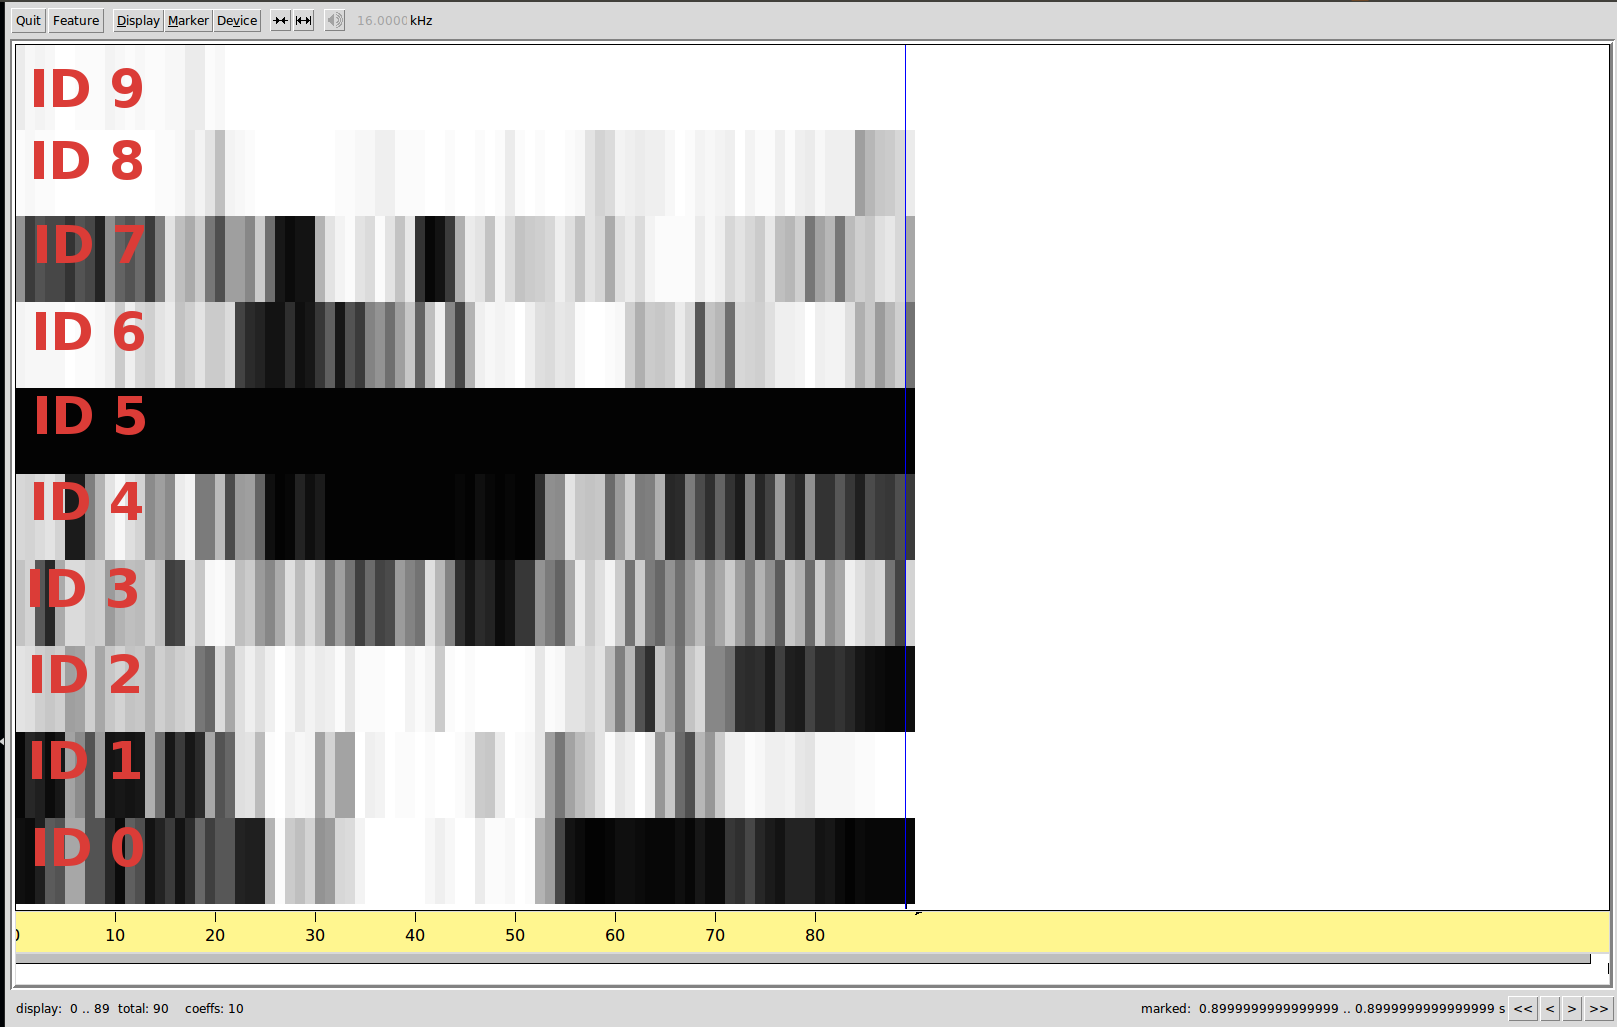
\includegraphics[width=0.7\textwidth]{images/polishCorrect.png}
\end{figure}

\begin{figure}[h!!]
\caption{Activation of output neurons for an incorrectly recognized English sample}
\label{fig:incorrect}
\centering
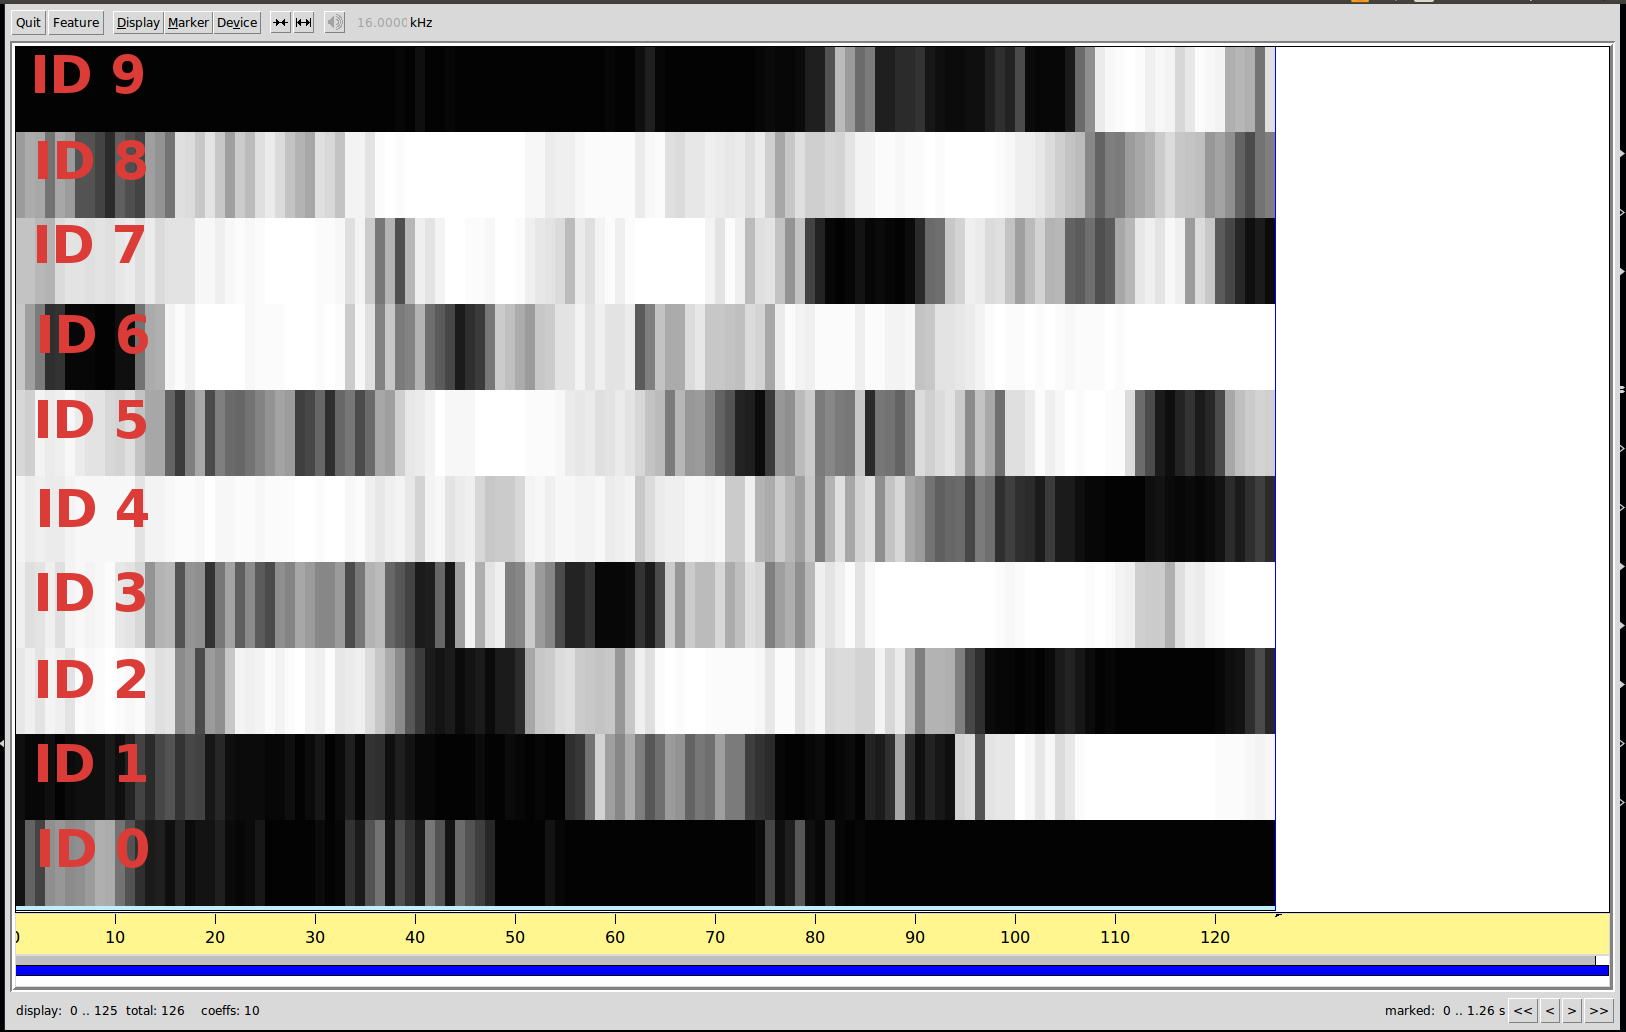
\includegraphics[width=0.7\textwidth]{images/incorrect.png}
\end{figure}
\newpage

\section{Evaluation Metric}
\label{sec:eval:bare}

To have a baseline to improve upon we evaluated the base net on full samples of differing lengths and then tried to improve these results. See app.~\ref{lst:basic} for the corresponding tcl/tk code for this bare approach. It counts a sample as correctly classified if the majority of frames/filtering steps have been classified correctly. The test setup used then goes through the entire set of samples and counts the correctly/wrongly classified samples for each language. This means that an extra amount of smoothing is included, but results should still be sufficiently general to be able to infer properties of employed filters, as they all include this extra smoothing.  This additional smoothing can be applied in an online fashion by setting a sufficiently large, while still small enough to not incur delay, window size and then counting the occurence of outputs to give the same effect as used here. 

\subsection{Out-Of-Language Error (OLE)}
\label{sec:eval:ole}

The first correctness metric proved to be too restrictive for filters. As filters might reduce the count of the correct language while making the total number of wrong outputs less, we present another metric to evaluate filter effectiveness. We count the total number of falsely (as in not-equal to the maximum output) classified frames/output per sample divided by the number of total frames/outputs and average them on a per-sample basis to see if filters actually work in filtering out false outputs. It basically gives a metric for the amount of noise the net output includes. Arguably this would be even more important in an online-fashion in the Lecture Translator, as wrong outputs/filters would be passed on to the speech recognition/translation APIs. This second metric evaluation for well-performing filters can be found at the end of the chapter in table~\ref{tab:evalTotal}.

\begin{table}[h!]
\centering
\caption{Results of different net structures evaluated on the Euronews DEV set.}
\label{tab:evalNS}
\begin{tabular}{| l | r |}
	\hline
	\textbf{Net Structure} & \textbf{Overall Error}  \\
	\hline
	6-layer tree-net lr 0.1 & 0.318 \\
	\hline
	6-layer tree-net  &  0.311 \\
	\hline
	7-layer tree-net & 0.316 \\
	\hline
\end{tabular}
\end{table}

The results of the bare-net evaluation for Euronews can be seen in table~\ref{tab:bareResults} for the best performing net structure, the 6-layered-tree-structure as introduced in sec.~\ref{sec:LIDNetwork:Layout}. The results are, as expected, worse than the frame-based training-recognition, as here the entire (not-yet seen) samples are run through the net.  fig.~\ref{fig:lengthBasic} shows the relation of the length of samples and the amount of correctly classified samples of this length for the tree-structure-net. It shows the intuitive results of a longer length of a sample coinciding with a higher recognition rate through the net, as more frames can be used for the recognition task in the context produced by the ASR BNF net. However, it is also evident that for samples with a length of only 17 frames (~200 ms), the net already categorizes the sample better than guessing a language (which on average would yield a correctness of 0.1), as for 17, the net produces a correctness of 0.1896.

As one can see a length of around 100 frames (meaning a sample length of: \(100*10 / 1000 = 1s \)) is sufficient to be able to recognize the language with a correctness of \(\approx\)70 \%. This means online recognition of language is possible with a relatively small warm-up time of 1 second (or around 2 seconds with a higher correctness of then well over 80 \%).
\begin{figure}[h!]
\label{fig:lengthBasic}
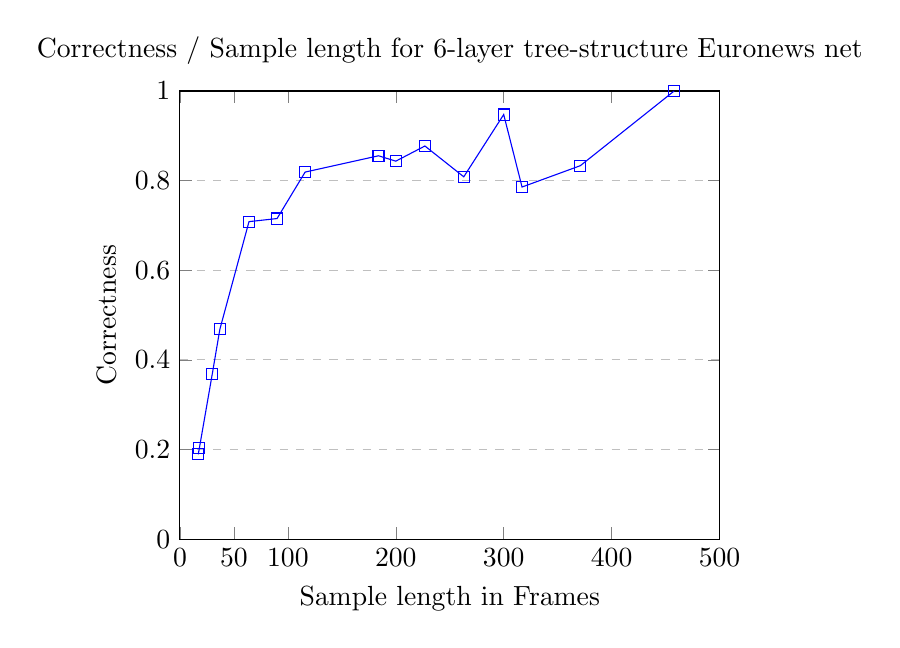
\begin{tikzpicture}
\begin{axis}[
	title={Correctness / Sample length for 6-layer tree-structure Euronews net},
	xlabel={Sample length in Frames},
	ylabel={Correctness},
	xmin=0, xmax=500,
	ymin=0, ymax=1,
	xtick={0,50,100,200,300,400,500},
	ytick={0,0.2,0.4,0.6,0.8,1},
	legend pos=north west,
	ymajorgrids=true,
	grid style=dashed,
]
\addplot[
	color=blue,
	mark=square,
	]
	coordinates {
	(17,0.1896)(18,0.2030)(30,0.3690)(37,0.4683)(64,0.7085)(90,0.7154)(116,0.8190)(184,0.8554)(200,0.8434)(227,0.8772)(263,0.8085)(300,0.9474)(317,0.7857)(371,0.8333)(458, 1)
	};
\end{axis}
\end{tikzpicture}
\end{figure}
\begin{table}[h!]
\caption{Results of the best net structure (tree-structure 6-layer) evaluated on the Euronews DEV with only bare net output.}
\label{tab:bareResults}
\centering
\begin{tabular}{| l | c | r | }
	\hline
	\textbf{Language} & \textbf{Error (total)}  & \textbf{Error (samples >500 ms)} \\
	\hline
	Arabian & 0.364 &  0.235 \\
	German & 0.300 &  0.155 \\
	Spanish & 0.320 & 0.155 \\ 
	French & 0.300  & 0.138 \\
	Italian & 0.326  & 0.174 \\
	Polish & 0.267 & 0.111 \\
	Portuguese& 0.291 & 0.161 \\
	Russian&  0.315 & 0.148 \\
	Turkish&  0.337 & 0.182 \\
	English&  0.267 &0.145\\
	\hline
	\textbf{Overall} & 0.267 & 0.162\\
	\hline
\end{tabular}
\end{table}

\section{Basic Test Filter}
\label{sec:eval:basic}

The first filter used was basic 5-Frame smoothing: It saves the value of the last direct outputs and only outputs a language if the last 5 direct outputs would have been the same. It also includes a filtering based on the actual output of the language ID neuron, only counting outputs higher than an arbitrarily defined activation of 0.61. However this can be disregarded, as for the vast majority of samples the maximum neuron for a certain frame never fell underneath this threshold.

This approach requires a 5 frame (\(\approx 50 ms\)) ``warm-up'' time, which still would make it usable in an online environment.

table~\ref{tab:basic} shows the result of the basic filter for each language. Overall the error (for our defined metric) went up by about 5 \%. It did however improve results for Arabian by about 3 \%, showing that the finding of a suitable filter that improves the overall recognition is non-trivial, as apparently some languages will benefit from a certain type of filter while another will not. 

\begin{table}[h!]
\centering
\caption{Results of the best net structure (tree-structure 6-layer) evaluated on the Euronews DEV Set with the Basic Filter.}
\label{tab:basic}
\begin{tabular}{| l | c | r | }
	\hline
	\textbf{Language} & \textbf{Error (total)}  \\
	\hline
	Arabian & 0.337  \\
	German & 0.312  \\
	Spanish & 0.331 \\ 
	French & 0.313 \\
	Italian & 0.334  \\
	Polish & 0.277 \\
	Portuguese& 0.310  \\
	Russian&  0.322 \\
	Turkish&  0.343 \\
	English&  0.286 \\
	\hline
	\textbf{Overall} & 0.318 \\
	\hline
\end{tabular}
\end{table}


\section{Advanced Test Filter}
\label{sec:eval:advanced}
The advanced test filter is based on the JRTk's \textit{FILTER} capability. It automatically takes a defined amount of frames and calculates the weighted arithmetic mean with predefined weights for incoming audio. First tries were done using a small filter setup of:
\begin{verbatim}
filter          nnFILTERSMALL   nnBNF  {-2 {1 2 3 2 1}}
\end{verbatim}  Herein the context is 2 frames on each side of the current frame (the first parameter) with weights 1, 2 , 3 , 2 , 1 for the 5 frames respectively.  It however offered no improvement of results, rather a decline in total correctness so different filter approaches were tried:
\begin{verbatim}
filter          nnFILTERBIG nnBNF {-5 {1 2 3 4 5 6 5 4 3 2 1}}
\end{verbatim}
which however did not provide a further increase in correctness. In our tcl filtering, we only then changed the feature to read the frames from, while still then taking the maximum of the filter-feature as the output. Comparison of the two filter can be seen  in table ~\ref{tab:evalAdvanced} for evaluation on the DEV set. As compared to the bare net output, the bigger advanced filter offered a tiny improvement for some languages, (~0.1\% for both Portuguese and English) in correctness but lost out in all other languages. Detailed per-Language results for this and the following filters can be found in app.~\ref{app:res:lid}.

\begin{table}[h!]
\centering
\caption{Results of the best net structure (tree-structure 6-layer) evaluated on the Euronews DEV Set with the Advanced FILTER}
\label{tab:evalAdvanced}
\begin{tabular}{| l | r |}
	\hline
	\textbf{Filter} & \textbf{Overall Error}  \\
	\hline
	Small FILTER  &  0.313 \\
	\hline
	Large FILTER & 0.316 \\
	\hline
\end{tabular}
\end{table}


\section{Difference Test Filter}
\label{sec:eval:variance}
As a next approach, the difference between the two most likely outputs was taken into account. We filtered the direct output by only changing from the previous output, if the difference (which we implied to be how sure the net was when determining the language) was bigger than 0.01. 

Aside from the general errors with the correctness metric as already outlined in the beginning of this chapter, we also thought one possible reason for a worse performance of this filter could be, that the output of the 2\textsuperscript{nd} most likely neuron is not going to differ from the maximum output on many language pairs: E.g. French/Italian, Russian/Polish, Italian/Portuguese,  even if the net predicts one over the other as the difference between the languages is also relatively ``small''. E.g as presented in~\cite{doi:10.1080/14790710508668395}, the difference between English and French is small as the ``linguistic score'' is relatively high with 2.5. 

The full tcl code of this filter can be found in the appendix . The evaluation results can be seen in tab.~\ref{tab:evalTotal}

\section{Counting Filter}
This filter included a counting of the occurrence of a certain net output in a frame-range, and then outputting the ID of the language that was recognized the most in that frame-range (while still then employing the same per-sample smoothing as above). The first try was done using a frame-range of 10, later increased further. We listed the results of this filter with different ranges on the DEV set in \ref{tab:counting}. As a further experiment we also used overlapping windows (meaning we count the occurrence in 10 frames and the next 10 frames are not 10 frames further but starts at the 8th frame of the previous window -> overlap of 3 frames).

The full code of this filter can be found in the Appendix.

\begin{table}[h!]
\caption{Results of the best net structure (tree-structure 6-layer) evaluated on the Euronews DEV Set with the Counting Window Filter}
\label{tab:counting}
\centering
\begin{tabular}{| l | r |}
	\hline
	\textbf{Filter} & \textbf{Overall Error}  \\
	\hline
	Counting Filter FR 10  & 0.313 \\
	\hline
	Counting Filter FR 10, overlap 3 &  0.323\\
	\hline
	Counting Filter FR 50 & 0.316 \\
	\hline
	Counting Filter FR 100 & 0.313\\
	\hline
	Counting Filter FR 150 & 0.314\\
	\hline
\end{tabular}

\end{table}

\section{Sequence Filter}
\label{sec:eval:seq}
This filter included a counting of the longest sequence of a certain net output in a frame-range, and then outputting the ID of the language that was recognized for the ongest sequence in that frame-range (while still then employing the same per-sample smoothing as above). This decreased the OLE substantially as can be see in table~\ref{tab:evalTotal}, however the filter did increase the overall error by 8\%, more than any of the other filters, 

The full code of this filter can be found in the Appendix.


\section{Two-Language Setup}
\label{sec:eval:2L}
table~\ref{tab:eval2L} shows the result produced by using the LID Euronews net for 10 languages on different combinations of 2 languages (namely French/Italian and English/German). In this case we ignore the output of the net if it doesn't equal one of the two languages and instead keep the previous output intact in this case. This, intuitively, gave a big boost in the recognition rate, bringing the rate up to 85 \% for the two languages combined, an improvement of more than 10 \% in correctness compared to the bare approach in sec.~\ref{sec:eval:bare}.

\begin{table}[h!]
\caption{Results of the best net structure (tree-structure 6-layer) evaluated on only 2 Languages with the 2-language filter on the DEV set.}
\label{tab:eval2L}
\centering
\begin{tabular}{| l | r |}
	\hline
	\textbf{Language} & \textbf{Error (total)}  \\
	\hline
	\textbf{French/Italian as input only} & \\
	 French &  0.186 \\
	Italian & 0.113 \\
	\hline
	\textbf{Overall} & 0.153 \\
	\hline
	\textbf{German/English as input only} & \\
	German & 0.183 \\
	English & 0.126 \\
	\hline
	\textbf{Overall} & 0.156 \\
	\hline
\end{tabular}
\end{table}

\section{Gaussian Smoothing Filter}
\label{sec:eval:GSF}
Gaussian filters have shown great success in the realm of image processing in the form of canny edge detectors. 
A one-dimensional Gaussian filter returns a response that is akin to the form of a normal distribution:
\begin{figure}[h!]
\centering
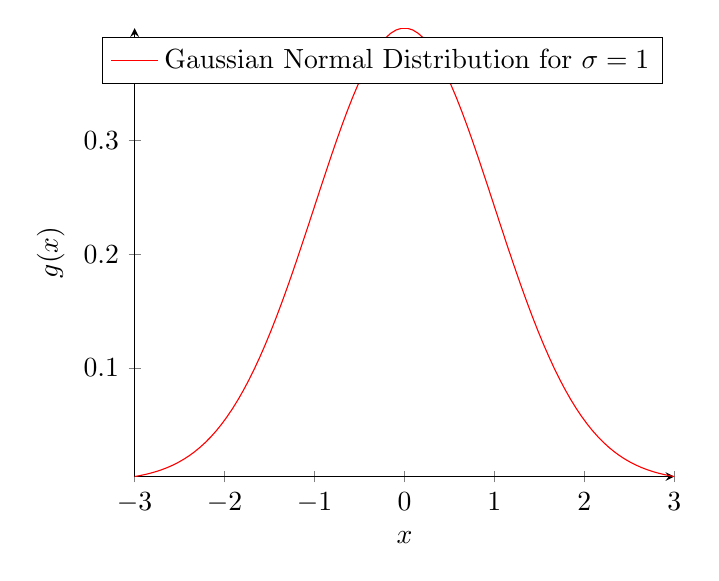
\begin{tikzpicture}
\begin{axis}[
	axis lines = left,
	xlabel = \(x\),
	ylabel = \(g(x)\),
]
\addplot[domain=-3:3,
		samples=100,
		color=red,
]
{1 / ((2 * pi)^0.5) * exp(- ((x^2) / 2))};
\addlegendentry{Gaussian Normal Distribution for \(\sigma = 1\)}
\end{axis}
\end{tikzpicture}
\end{figure}
To calculate the Gaussian Filter Response, one needs a Gaussian Kernel with a Window-Size. While in general the Gaussian filter has an infinite window size, choosing a fixed window size can approximate the Gaussian well. In this discrete case \(\sigma\), the standard deviation of the Gaussian, can be approximated with \(N\) the size of the window:
\begin{equation}
\sigma  =\sqrt{\frac{N}{2\pi}}
\end{equation}
With \(\sigma\), the Gaussian function for point \(x\) can be calculated as:
\begin{equation}
g(x) = \frac{1}{\sqrt{2\pi}\sigma} * e^{{- \frac{x^2}{2\sigma^2}}}
\end{equation}
Once the Gaussian function is calculated for the window, the convolution of the data points with the Gaussian kernel is performed, resulting in smoothed over coefficients of the LID net output. The maximum smoothed coefficient is then chosen and the corresponding language is output, which gave us definite improvements over the unsmoothened net output. In tcl the relevant code part can be seen in~\ref{lst:tclGauss}, in which we presume the window size to mean the number of points we take into account on both sides of the origin, while normally this number is the window size - 1.


We tried different window sizes of which the result can be seen in tab.~\ref{tab:evalGauss} on the DEV Set.  As can be seen, the Window size of 15 performed the best out of the different window sizes evaluated. To showcase a correct implementation fig.~\ref{fig:gaussWS10} shows the result of one Gaussian convolution for a window size of 10 as a graph, as one can see it is evident that the graph looks similar to the Gaussian kernel as graphed above and smoothing of the data has evidently occurred.  As it turns out the Gauss Filter indeed performs much better even on the correctness-metric on small samples with a size under 50 frames (=500ms). tab.~\ref{tab:50Gauss} showcases this in comparison to the bare net output, which shows a very significant improvement of 15\%.

\begin{figure}
\label{fig:gaussWS10}
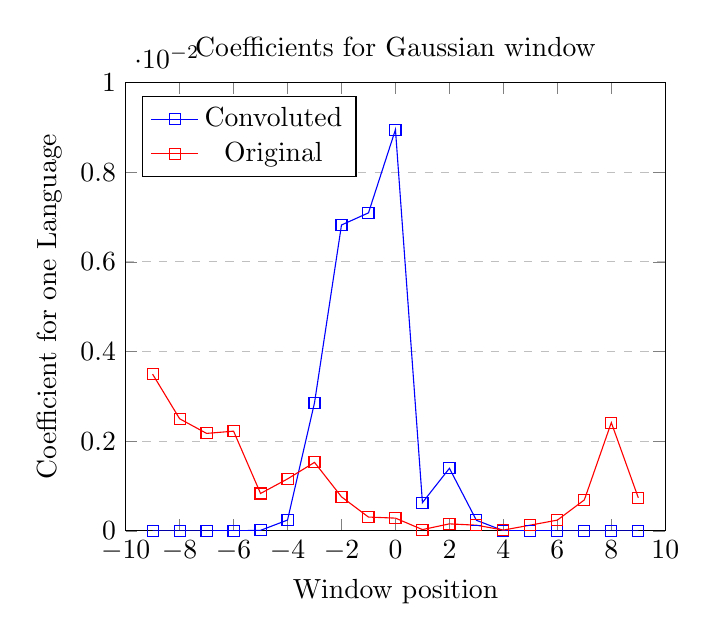
\begin{tikzpicture}
\begin{axis}[
	title={Coefficients for Gaussian window},
	xlabel={Window position},
	ylabel={Coefficient for one Language},
	xmin=-10, xmax=10,
	ymin=0, ymax=0.01,
	xtick={-10,-8,-6,-4,-2,0,2,4,6,8,10},
	ytick={0,0.002,0.004,0.006,0.008,0.01},
	legend pos=north west,
	ymajorgrids=true,
	grid style=dashed,
	legend entries = {Convoluted, Original}
]
\addplot[
	color=blue,
	mark=square,
	]
	coordinates {
	(-9,0.000000000000981436047264734)(-8,0.000000000146530269711589)(-7,0.0000000141764935038566)(-6,0.000000861340018697172)(-5,0.0000102217155818498)(-4,0.000240166306972279)(-3,0.002856375317948)(-2,0.006821435047423)(-1,0.007091839168043)(0,0.008949052879339)(1,0.000628630253053)(2,0.001394595714444)(3,0.000234592882892)(4,3.42E-06)(5,1.56E-06)(6,9.24E-08)(7,4.50E-09)(8,1.41E-10)(9,2.07E-13)
	};
\addplot[
	color=red,
	mark=square,
	]
	coordinates {
	(-9,3.493900E-03)(-8,2.499977E-03)(-7,2.172766E-03)(-6,2.222949E-03)(-5,8.326542E-04)(-4,1.157482E-03)(-3,1.526701E-03)(-2,7.579251E-04)(-1,3.070411E-04)(0,2.829939E-04)(1,2.721654E-05)(2,1.549526E-04)(3,1.253873E-04)(4,1.650676E-05)(5,1.267841E-04)(6,2.384537E-04)(7,6.895550E-04)(8,2.413667E-03)(9,7.368696E-04)
	};
\end{axis}
\end{tikzpicture}
\end{figure}

\begin{table}[h!]
\caption{Results of the 6-layer tree-structure evaluated with different Gauss filters on the DEV set.}
\label{tab:evalGauss}
\centering
\begin{tabular}{| l | r |}
	\hline
	\textbf{Filter} & \textbf{Overall Error}  \\
	\hline
	Gaussian Filter WS 10 & 0.3128 \\
	\hline
	Gaussian Filter WS 15 & 0.3125 \\
	\hline
	Gaussian Filter WS 17 & 0.3126 \\
	\hline
	Gaussian Filter WS 20 & 0.3130 \\
	\hline
\end{tabular}
\end{table}

\begin{table}[h!]
\caption{Comparison of results of the 6-layer tree-structure evaluated on DEV set for small samples.}
\label{tab:50Gauss}
\centering
\begin{tabular}{| l | r |}
	\hline
	\textbf{Filter} & \textbf{Overall Error (< 500 ms)}  \\
	\hline
	Bare Net Output & 0.590 \\
	\hline
	Gaussian Filter WS 15 & 0.439 \\
	\hline
\end{tabular}
\end{table}

\section{Speech Filter}
\label{sec:speech}

As described in Chapter~\ref{ch:FP} we extract a SPEECH feature from the input audio using the Sound power as a basis. In a further attempt to smooth output we used this to ignore any non-speech marked frames for output-calculation. This only gave us an error of around 0.02\% higher compared to the bare net output, however the filtering effectiveness (OLE) was worse than for the other filters as can be seen in \ref{tab:evalTotal}. 

\begin{table}[h!]
\caption{Results of the 6-layer tree-structure evaluated on samples longer than 50 frames (~500 ms)}
\label{tab:evalTotal2}
\centering
\begin{tabular}{| l | r |}
	\hline
	\textbf{Filter} & \textbf{Error (>500 ms) on DEV}  \\
	\hline
	 Bare Net & 0.162 \\
	\hline
	Counting Filter FR 10 & 0.178\\
	\hline
	Speech/Noise Filter & 0.163\\
	\hline
\end{tabular}
\end{table}


\begin{table}[h!]
\centering
\caption{Results of the 6-layer tree-structure evaluated with all the tried post-filtering approaches on both the DEV and TEST set.}
\label{tab:evalTotal}
\begin{tabular}{| l | c | r |}
	\hline
	\textbf{Filter} & \textbf{Overall Error DEV/TEST} & \textbf{OLE DEV/TEST} \\
	\hline
	Bare Net & 0.311/0.305 & 0.202/0.198 \\
	\hline
	Advanced Filter (small) & 0.318/0.312 & 0.185/0.181 \\
	\hline
	Difference & 0.317/0.311 & 0.170/0.165 \\
	\hline
	Gaussian Filter (WS 15) & \textbf{0.313}/0.307  & 0.181/0.176 \\
	\hline
	Counting Filter (WS 100) & \textbf{0.313}/0.307 & \textbf{0.007/0.006} \\
	\hline
	Speech/Noise Filter  & \textbf{0.313/0.306} & 0.187/0.181 \\
	\hline
	English/German &  0.116/0.216 & 0.145/0.166 \\
	\hline
	French/Italian & 0.207/0.214 &  0.158/0.159 \\
	\hline
	Sequence Filter (WS 10) & 0.393/0.382 & 0.031/0.029 \\
	\hline
	\textbf{Best (w/o 2L, Bare)} & \textbf{0.313/0.306} & \textbf{0.007/0.006} \\
	\hline
\end{tabular}

\end{table}

\section{Filter Selection}
\label{sec:eval:filterSelection}

Overall we conclude, that selection of a good filter is  a non-trivial problem, as already we saw that some filters perform better for certain languages or setups while suffering for others. Overall, our net performs reasonably well with all filters, reaching error of less than 20 \% for samples of length > 500 ms (See tab.~\ref{tab:evalTotal2}), a delay that would still make online-usage feasibly. On 10 target languages, using the Counting Filter with a Window size of 100 (so a delay of 1 second), would arguably perform the best while still filtering out the maximum of wrong outputs, featuring an OLE of only 0.007, a relative improvement of \((0.202-0.007) / 0.185 = 0.97 = 97 \% \) for the DEV set and \( 0.198- 0.006)/ 0.198 = 0.97 = 97\% \) compared to the bare net output.

For less delay, one could also implement the Sequence Filter for a small Window size of 10, which also gives us an relative improvement of \((0.202-0.031) / 0.202 = 0.85 = 85 \%\) on the DEV and \((0.198 - 0.031) / 0.198 = 0.84 = 84\% \) on the TEST set. However, this filter is likely to possibly change the overall output. However a combination of the Sequence and the Counting Filter on smaller window sizes might be feasible.

The Gauss Filter might also be a feasible choice as it improved results for very short samples (< 500 ms) and less jumps in the output of the Lecture Translator would be preferable, however the computational complexity of this filter is much higher compared to the other filters which might have to be taken into account in an online-environment.

Overall, in the lecture-translator environment, less target languages are likely, and so the language-filter for the correct amount of target languages would most likely be sufficient. However, further filtering on top of this will most likely decrease the amount of wrong output.

\section{Lecture-Data Evaluation}
\label{sec:eval:LD}

We added the same filtering as for the 2-language setup, ignoring non-available languages which improved the error by about 0.5 \% for the tree-net, giving an overall error of 0.175 instead of the 0.179. See tab.~\ref{tab:resultsLD2l}


\begin{table}[h!]
\caption{Results of the 6-layer tree-structure evaluated on lecture data (LD) DEV samples.}
\label{tab:resultsLD2l}
\centering
\begin{tabular}{| l | r |}
	\hline
	\textbf{Filter} & \textbf{Error}  \\
	\hline
	 Bare Net & 0.179 \\
	\hline
	3L-Filter & 0.175\\
	\hline
\end{tabular}
\end{table}





	